\documentclass{standalone}
\usepackage{tikz}
\usepackage{pgfplots}
\pgfplotsset{width=32cm,height=18cm,compat=1.3}
\pgfplotsset{every tick label/.append style={font=\Huge}}
\usepackage{filecontents}

\usetikzlibrary{patterns}

\definecolor{citrine}{rgb}{0.89, 0.82, 0.04}

\begin{document}
	\centering
		\vspace{1.5em}
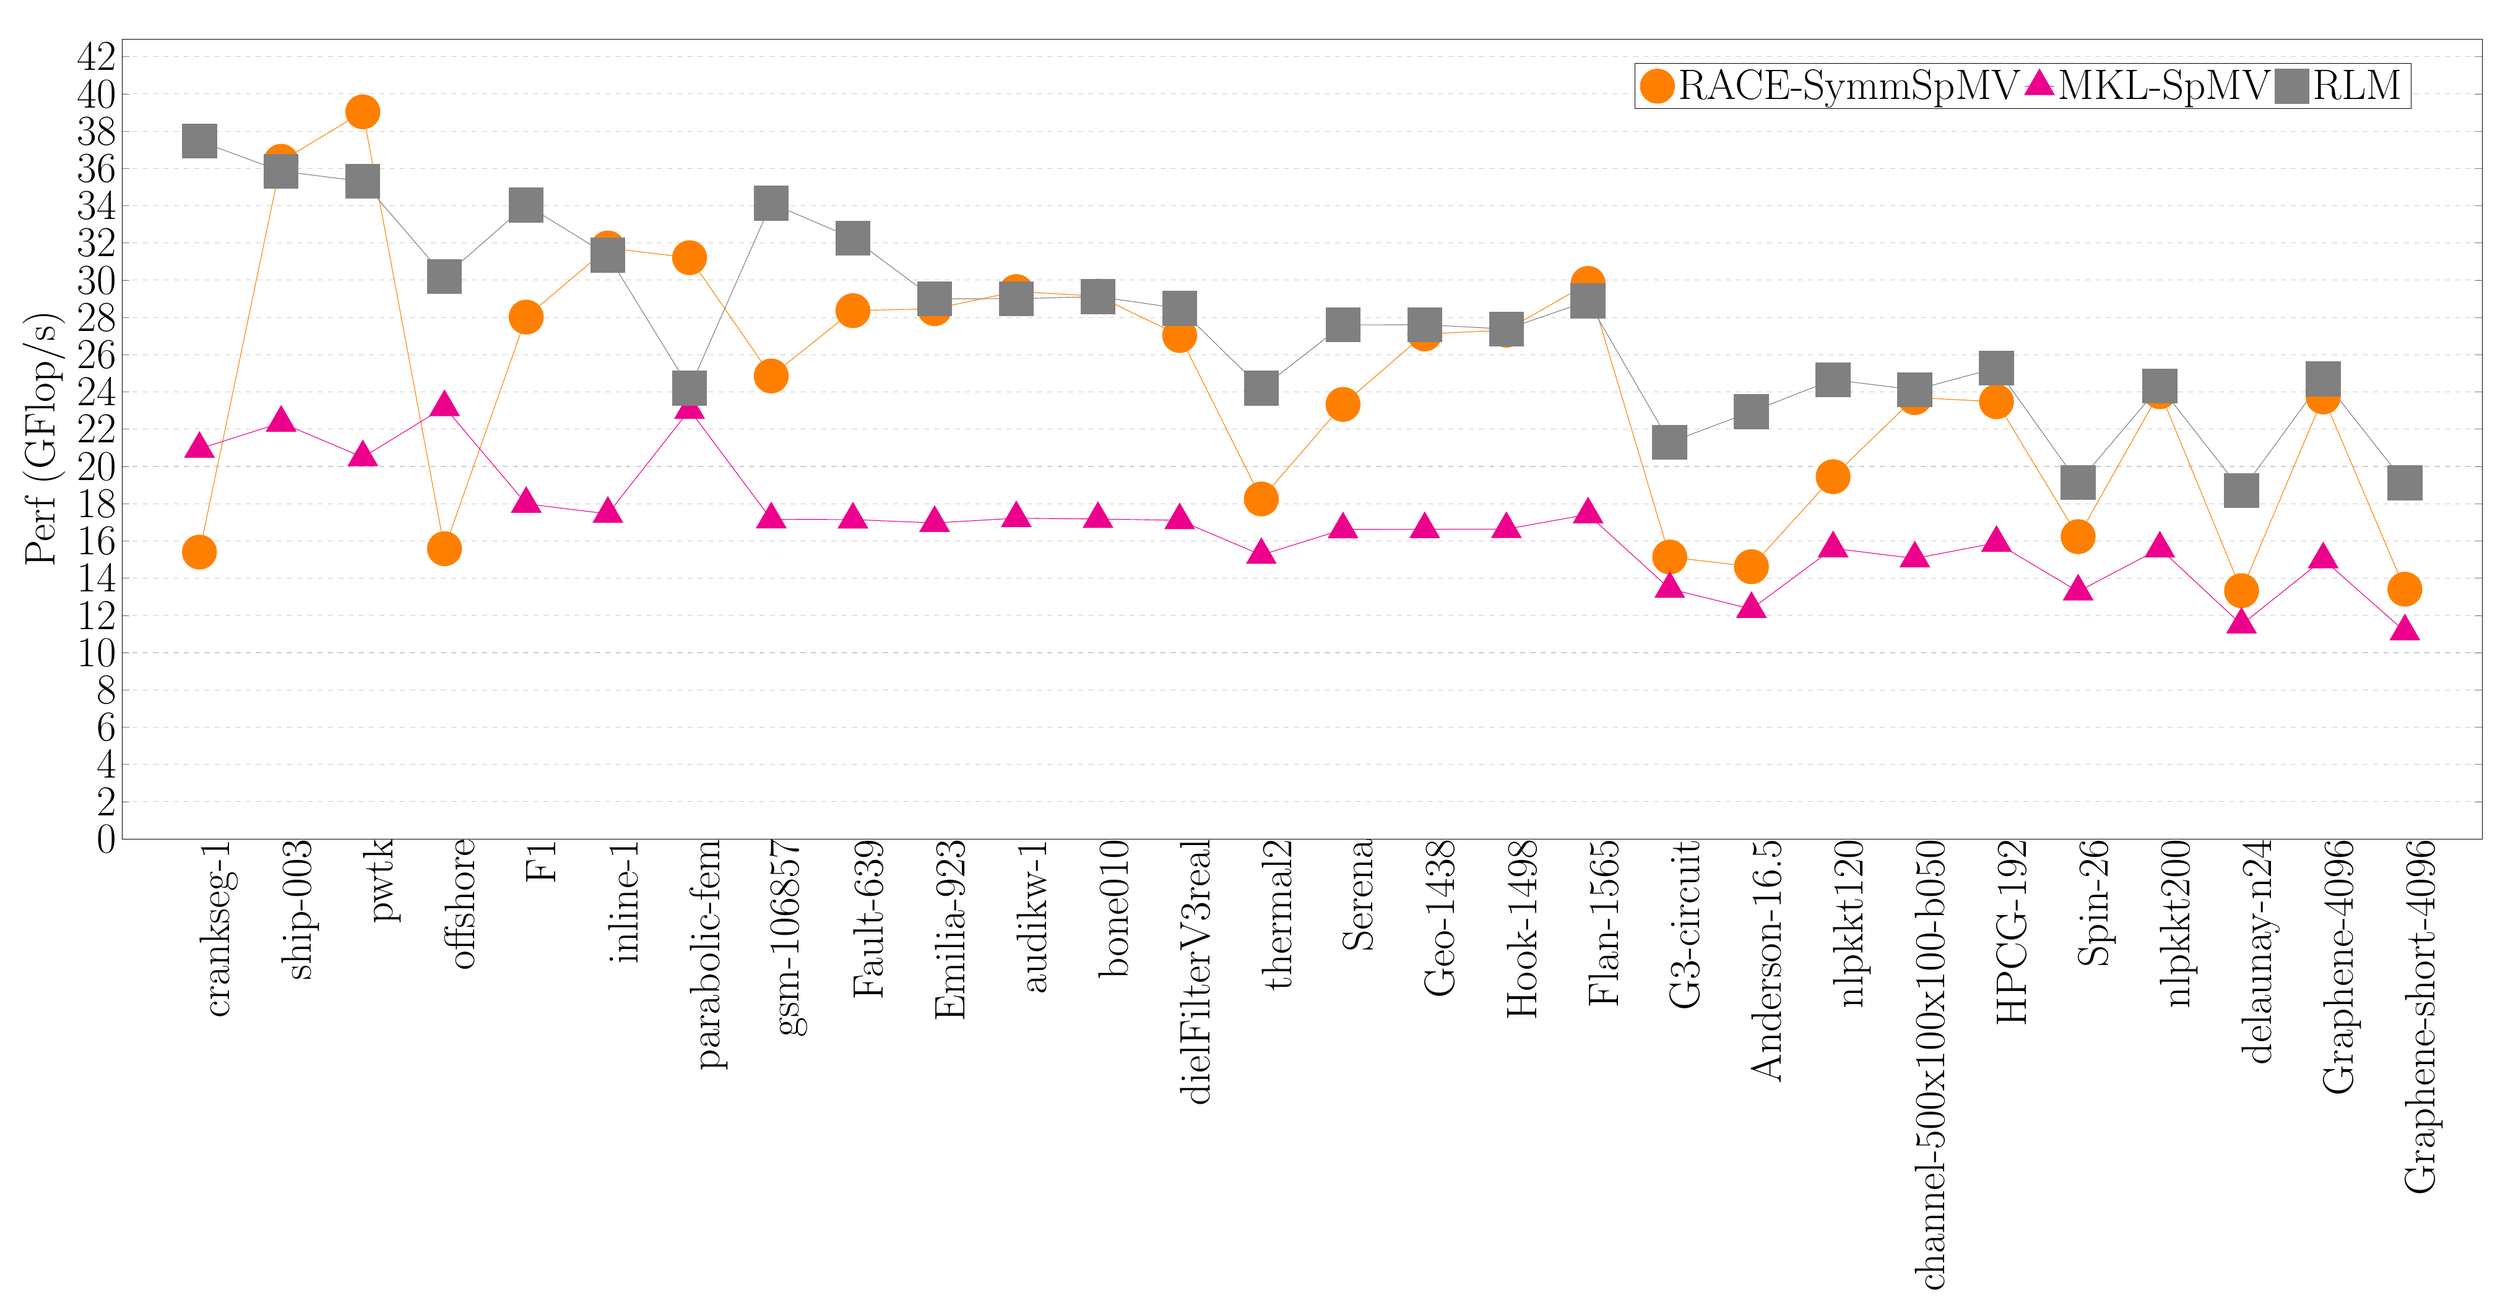
\begin{tikzpicture}
		%	\node at (13.25,15) {\LARGE{}};
			\begin{axis}[
		%	xmin=0.25, xmax=7.25,
			ymin=0, %ymax=3.25,
			xtick={1, 2, 3, 4, 5, 6, 7, 8, 9, 10, 11, 12, 13, 14, 15, 16, 17, 18, 19, 20, 21, 22, 23, 24, 25, 26, 27, 28},
		%	ytick={0,0.5,1,1.5,2,2.5,3},
			xticklabels={crankseg-1, ship-003, pwtk, offshore, F1, inline-1, parabolic-fem, gsm-106857, Fault-639, Emilia-923, audikw-1, bone010, dielFilterV3real, thermal2, Serena, Geo-1438, Hook-1498, Flan-1565, G3-circuit, Anderson-16.5, nlpkkt120, channel-500x100x100-b050, HPCG-192, Spin-26, nlpkkt200, delaunay-n24, Graphene-4096, Graphene-short-4096},
			width  = 50cm,
			height = 18cm,
			major x tick style = transparent,
			%	minor ytick={1, 5, 10, 15, 20, 25, 30 ,35,40},
			grid = minor,	
			%add_bar_commands
			ymajorgrids = true,
			grid style={dashed, gray!40},
			ylabel = {\Huge{Perf (GFlop/s)}},
		%	symbolic x coords={Graphene-2048-2048, Graphene-4096-4096, Spin-24-24-24},
			x tick label style={rotate=90, anchor=north east, inner sep=0mm, font={\Huge}},
			tick label style={font={\Huge}},
			scaled y ticks = false,
			enlarge x limits=0.035,
			legend cell align=left,
			legend style={font=\Huge},
			legend columns=-1,
			legend style={
				%at={(1,1.05)},
				%anchor=south east,
				%column sep=1ex,
				legend pos=north east
			},
			%spl_legend_code
			title= {\Huge\scalebox{1.5}{{}}}
			]

\addplot[mark=*, mark size=10pt, mark options={orange}, draw=orange ] plot coordinates{(1,15.400558) (2,36.382835) (3,39.039620) (4,15.581563) (5,28.019140) (6,31.731108) (7,31.206720) (8,24.857203) (9,28.363801) (10,28.469068) (11,29.389081) (12,29.144620) (13,27.028246) (14,18.254121) (15,23.331850) (16,27.115273) (17,27.315481) (18,29.827848) (19,15.135629) (20,14.616334) (21,19.448762) (22,23.696725) (23,23.475947) (24,16.228225) (25,24.014094) (26,13.326586) (27,23.728702) (28,13.406762)};
\addplot[mark=triangle*, mark size=10pt, mark options={magenta}, draw=magenta ] plot coordinates{(1,20.943491) (2,22.344883) (3,20.492832) (4,23.182222) (5,17.990928) (6,17.452555) (7,23.036871) (8,17.155262) (9,17.146120) (10,16.964412) (11,17.219620) (12,17.176485) (13,17.105925) (14,15.245571) (15,16.616126) (16,16.627225) (17,16.633843) (18,17.422747) (19,13.421811) (20,12.344783) (21,15.602316) (22,15.057594) (23,15.898243) (24,13.281274) (25,15.589733) (26,11.502923) (27,15.008665) (28,11.138126)};
\addplot[mark=square*, mark size=10pt, mark options={gray}, draw=gray ] plot coordinates{(1,37.467821035188415) (2,35.851973903808435) (3,35.304185482391006) (4,30.201212426199582) (5,34.03975592170131) (6,31.341638554379703) (7,24.197426270643927) (8,34.132154737070024) (9,32.24996046983436) (10,28.997431933741016) (11,29.008041555231586) (12,29.11716671941068) (13,28.48354715618585) (14,24.19598370828887) (15,27.598818685423954) (16,27.60950248602838) (17,27.37761544023837) (18,28.87732441334738) (19,21.293955821929345) (20,22.938936550901495) (21,24.65850056358395) (22,24.111193475848093) (23,25.28320447161289) (24,19.12829106406081) (25,24.30914431812) (26,18.695319384101396) (27,24.69259765674899) (28,19.120795826479952)};
	%addplot cmd

	\legend{RACE-SymmSpMV, MKL-SpMV, RLM}

	\end{axis}			
\end{tikzpicture}

\end{document}

